\chapter{Flow of Association And Causation in Graphs}
\section{Bayesian Networks and Causal Graphs}
Assume we only care about modeling association, without any causal modeling. If
we want to model the data distribution $P(X_1, X_2, \ldots, X_n)$, we can use
the chain rule of probability to decompose it into a product of conditional
distributions:
\begin{equation}
    P(X_1, X_2, \ldots, X_n) = P(X_1) \cdot P(X_2|X_1) \cdot \ldots \cdot P(X_n|X_1,
    \ldots, X_{n-1}) = P(X_1) \cdot \prod_{i=2}^n P(X_i|X_1, \ldots, X_{i-1})
\end{equation}
However, if we were to model discrete random variables by using probability
tables, it would take an exponential number of parameters. To solve this we
can model local dependencies between variables to reduce the number of
parameters.

\begin{definition}[\textbf{Local Markov Assumption}]
    Given all the parents $pa(x)$ of a node $x$ in a DAG, the local Markov
    assumption states that $x$ is independent of all its non-descendants.
\end{definition}
Talking about Bayesian networks, the local Markov assumption is equivalent to
the \textbf{bayesian network factorization}:
\begin{equation}
    P(X_1, X_2, \ldots, X_n) = \prod_{i=1}^n P(X_i|pa(X_i))
\end{equation}

At this point we can define a \textbf{Markov Probability Distribution} as a
probability distribution $P$ that satisfies the local Markov assumption with
respect to a DAG $G$.

As important as the local Markov assumption is, it only gives us information
about the independencies in $P$ that a DAG $G$ implies.

To get this guaranteed dependence between adjacent nodes, we will generally
assume a slightly stronger assumption than the local Markov assumption, called
the \textbf{minimality assumption}.
\begin{definition}[\textbf{Minimality Assumption}]
    The minimality assumption means:
    \begin{enumerate}
        \item \textbf{local markov assumption}: Given all the parents $pa(x)$ of
              a node $x$ in a DAG, the local Markov assumption states that $x$
              is independent of all its non-descendants.
        \item Adjacent nodes in the DAG $G$ are dependent.
    \end{enumerate}
\end{definition}

Because removing edges in a Bayesian network is equivalent to adding independencies,
the minimality assumption is equivalent to saying that we can't remove any more
edges from the graph $G$.

\begin{definition}
    $P$ and $G$ are Markov Compatible if $P$ factorize according to $G$.
\end{definition}

Up to now all we presented was about statistical models and modeling association.
We now need to introduce some \textit{causal assumptions}, turn them into causal
models for allowing the study of causation. In order to introduce causal assumptions,
we must first understand what it means for $X$ to be a cause of $Y$. We can simply
define \textbf{cause} as follows:
\begin{definition}[\textbf{Cause}]
    $X$ is a cause of $Y$ if changing $X$ changes $Y$.
\end{definition}

Also, we can define \textbf{(strict) causal edges assumption} in a DAG $G$ as
every parent is a direct cause of all its children. Given this assumption, we can
define a \textbf{Causal graph} as a DAG $G$ that satisfies the strict causal edges
assumption.

Adding the causal edges assumption, implies that directed paths in the DAG take
on a very special meaning; they correspond to \textbf{causation}. This is in
contrast to other paths in the graph, which association may flow along, but
causation certainly may not.
\section{Chains, Forks, and Colliders}
To understand the difference between association flow and causal flow in DAGs,
we need the following minimal building blocks:
\begin{itemize}
    \item Two un-connected nodes;
    \item Two connected nodes;
    \item Chain;
    \item Fork;
    \item Collider.
\end{itemize}

By \textit{flow of association}, we mean whether any two nodes in a graph are
associated or not associated. In other terms, we want to know whether two nodes
are (statistically) dependent or (statistically) independent. However, we will
also study whether two nodes are conditionally independent or not.
\subsection{Two un-connected nodes}
Given a graph consisting of just two unconnected nodes, as reported in Figure~\ref{fig:two_unconnected_nodes},
these nodes are not associated, because there is no edge between them. To show
this, consider the factorization of the joint probability $P(X, Y)$ that the
Bayesian network factorization gives us: $P(X, Y) = P(X)P(Y)$. This factorization
immediately gives us a proof that the two nodes are unassociated (independent).

\begin{figure}[!ht]
    \centering
    
\includegraphics[width=0.2\textwidth]{img/flow/two_unconnected_nodes.png}
    \caption{Two unconnected nodes}
    \label{fig:two_unconnected_nodes}
\end{figure}
\subsection{Two connected nodes}
On the contrary, if there is an edge between the two nodes, as reported in Figure~\ref{fig:two_connected_nodes},
then the two nodes are associated. We exploit the causal edges assumption which
means that $X$ is a direct cause of $Y$. They are dependent and conditional dependent.

\begin{figure}[!ht]
    \centering
    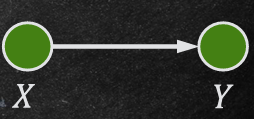
\includegraphics[width=0.2\textwidth]{img/flow/two_connected_nodes.png}
    \caption{Two connected nodes}
    \label{fig:two_connected_nodes}
\end{figure}

\subsection{Chain and Fork}
We can consider this two building blocks together, because they share the same
set of dependencies. In both cases, the association flows from $X$ to $Z$ through
$Y$.

They also share the same set of independencies. When we condition on $Y$ in both
graphs, it blocks the flow of association from $X$ to $Y$. Therefore, when we
condition on $Y$ ( $Z$'s parent in both graphs), $Z$ becomes independent of (and
viceversa). This independence is an instance of a \textbf{blocked path}.

\begin{figure}[!ht]
    \centering
    \begin{subfigure}[b]{0.45\textwidth}
        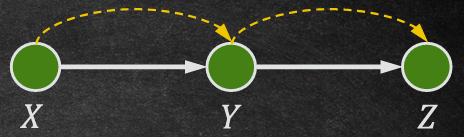
\includegraphics[width=\textwidth]{img/flow/chain.png}
        \caption{Chain}
        \label{fig:chain}
    \end{subfigure}
    \hfill
    \begin{subfigure}[b]{0.45\textwidth}
        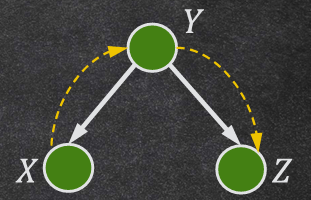
\includegraphics[scale=0.5]{img/flow/fork.png}
        \caption{Fork}
        \label{fig:fork}
    \end{subfigure}
\end{figure}

\begin{note}
    The flow of association in general is symmetric, but the flow of causation
    is not.
\end{note}
\subsection{Collider}
Association flows along any path that does not contain a \textbf{collider}. A
collider is a node with two or more parents that are independent $X \perp Z$, as
shown in Figure~\ref{fig:collider}. We can think of $X$ and $Z$ simply as unrelated
events that can happen, and which both contribute to some common effect ($Y$).
To show that $X \perp Z$ we apply the Bayesian network factorization and then
marginalize out $Y$.

\begin{figure}[!ht]
    \centering
    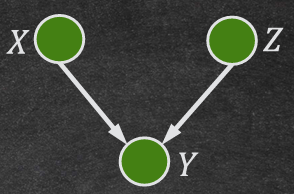
\includegraphics[width=0.2\textwidth]{img/flow/collider.png}
    \caption{Collider}
    \label{fig:collider}
\end{figure}

The collider $Y$ blocks the path from node $X$ to node $Z$ and blocks the path
from node $Z$ to node $X$. This is another example of a blocked path, but this
time the path is not blocked by conditioning; the path is un-blocked by conditioning
on a collider.

Conditioning on descendants of a collider also induces association in between the
parents of the collider. The intuition is that if we learn something about a
collider's descendant, we usually also learn something about the collider itself
because there is a direct causal path from the collider to its descendants, and
we know that nodes in a chain are usually associated assuming minimality.
\section{d-separation}
\begin{definition}[\textbf{d-separation}]
    A path $p$ is blocked by a set of nodes $\mathbb{S}$ if and only if:
    \begin{itemize}
        \item $p$ contains a \textit{chain} of nodes or a \textit{fork} such that
              the middle node is in $\mathbb{S}$.
        \item $p$ contains a \textit{collider} such that the collision node is
              not in $\mathbb{S}$, and no descendant of the collision node is in
              $\mathbb{S}$.
    \end{itemize}
    If $\mathbb{S}$ blocks \textbf{every} path between two nodes $X$ and $Y$, then
    $X$ and $Y$ are \textbf{d-separated}, conditional on $\mathbb{S}$, and thus
    are independent conditional on $\mathbb{S}$.
\end{definition}
D-separation is an extremely important concept, because it implies conditional
independence. This is a very powerful tool for reasoning about causal models.
\begin{itemize}
    \item $X \perp_G Y | \mathbb{S}$ implies that $X$ and $Y$ are d-separated in the DAG
          $G$ when conditioning on $\mathbb{S}$.
    \item $X \perp_P Y | S$ implies that $X$ and $Y$ are independent in the
          distribution $P$ when conditioning on $\mathbb{S}$.
\end{itemize}
\begin{definition}[\textbf{Global Markov Assumption}]
    Given that $P$ is Markov with respect to a DAG $G$, if $X$ and $Y$ are d-separated
    in $G$ conditional on $\mathbb{S}$, then $X$ and $Y$ are independent conditional
    on $\mathbb{S}$.
\end{definition}

Not only is association not causation, but causation is a sub-category of association,
thus association and causation both flow along directed paths.

We can tell if two nodes are not associated by whether or not they are d-separated.

If we want to measure the causal effect of $X$ on $Y$, we need to ensure that $X$
and $Y$ are d-separated in the augmented graph where we remove outgoing edges
from $X$. This is the only way to ensure that the association we measure is causation.

\begin{note}
    Association is symmetric while causation not.
\end{note}

To summarize the assumptions we made:
\begin{itemize}
    \item local/global Markov Assumption: tells us which nodes are unassociated,
          tells along which paths the association doesn't flow.
    \item Minimality assumption: tells us which paths association does flow along
    \item Causal edges assumption: tells us causation flows along directed paths.
\end{itemize}
\begin{figure}[!h]
    \centering
    \includegraphics*[width=\textwidth]{img/flow/causal_networks_assumptions.png}
    \caption{Causal networks assumptions}
    \label{fig:causal_networks_assumptions}
\end{figure}

